\documentclass{beamer}
%\usetheme{Copenhagen}
%\usetheme{Boadilla}
\usepackage{geometry}                % See geometry.pdf to learn the layout options. There are lots.
\usepackage{graphicx}
\usepackage{amssymb}
\usepackage{beamerthemeshadow}
 \usepackage{feynmp}
 \usepackage{textpos}
 \usepackage{biblatex}
 \usepackage{bbold}

  \usepackage{ulem}
  \usepackage{amsmath,amssymb} 
 \bibliography{foo}
  \DeclareGraphicsRule{*}{mps}{*}{} 
  % figures
  
 % \logo{
\includegraphics[height=1.2cm]{lhcblogo.jpg}\vspace{220pt}}
  
  
\usepackage{caption}
\usepackage{subfig}
\newcommand{\Lagr}{\mathcal{L}}
\setbeamertemplate{itemize item}{\scriptsize\raise1.25pt\hbox{\donotcoloroutermaths$\blacktriangleright$}}
\setbeamertemplate{itemize subitem}{\tiny\raise1.5pt\hbox{\donotcoloroutermaths$\square$}}
\setbeamertemplate{itemize subsubitem}{\tiny\raise1.5pt\hbox{\donotcoloroutermaths$\blacktriangleright$}}
\setbeamertemplate{enumerate item}{\insertenumlabel.}
\setbeamertemplate{enumerate subitem}{\insertenumlabel.\insertsubenumlabel}
\setbeamertemplate{enumerate subsubitem}{\insertenumlabel.\insertsubenumlabel.\insertsubsubenumlabel}
\setbeamertemplate{enumerate mini template}{\insertenumlabel}
\begin{document}
{


\title[$\Lambda_{b} \rightarrow p \mu \nu$ Form Factors \hspace{2em}\insertframenumber/
\inserttotalframenumber]{$\Lambda_{b} \rightarrow p \mu \nu$ Form Factors}
\author[William Sutcliffe]{
\includegraphics[height=1cm,width=1.5cm]{lhcblogo.jpg} \\ William Sutcliffe \\ \vspace{0.5cm} Imperial College London}



\date{\today}


 \frame{\titlepage

} 

\addtobeamertemplate{frametitle}{}{%
\begin{textblock*}{100mm}(.85\textwidth,-1cm)

\includegraphics[height=1cm,width=1.5cm]{lhcblogo.jpg}
\end{textblock*}}

 %%%%slide 1

% \frame{\frametitle{Outline} 
%\begin{enumerate}
%\setlength{\itemsep}{10pt}
%\item Background and motivation.
%\item Previous measurements.
%\item $V_{ub}$ with LHCb
%\item Initial generator level study
%\end{enumerate}
%}




%\frame{\frametitle{Table of contents}\tableofcontents} 

%\section{Context and Motivation}


\section{$\Lambda_{b} \rightarrow p \mu \nu$ Form Factors}
  \frame{
 \frametitle{$\Lambda_{b} \rightarrow p \mu \nu$ Form Factors}
 The tree-level matrix element for this decay may be written as:
\[
 \mathcal{M} =  -i \frac{G_{F}}{\sqrt{2}} V_{ub} H_{\nu} \overline{u}_{\mu} \gamma^{\nu} (1 - \gamma_{5}) v_{\nu_{\mu}}
\]
 where $H_{\nu} = <N^{+}(p',s')|\overline{u} \gamma_{\nu} (1 - \gamma_{5}) b | \Lambda^{0}_{b}(p,s)>$ 
  \begin{center}
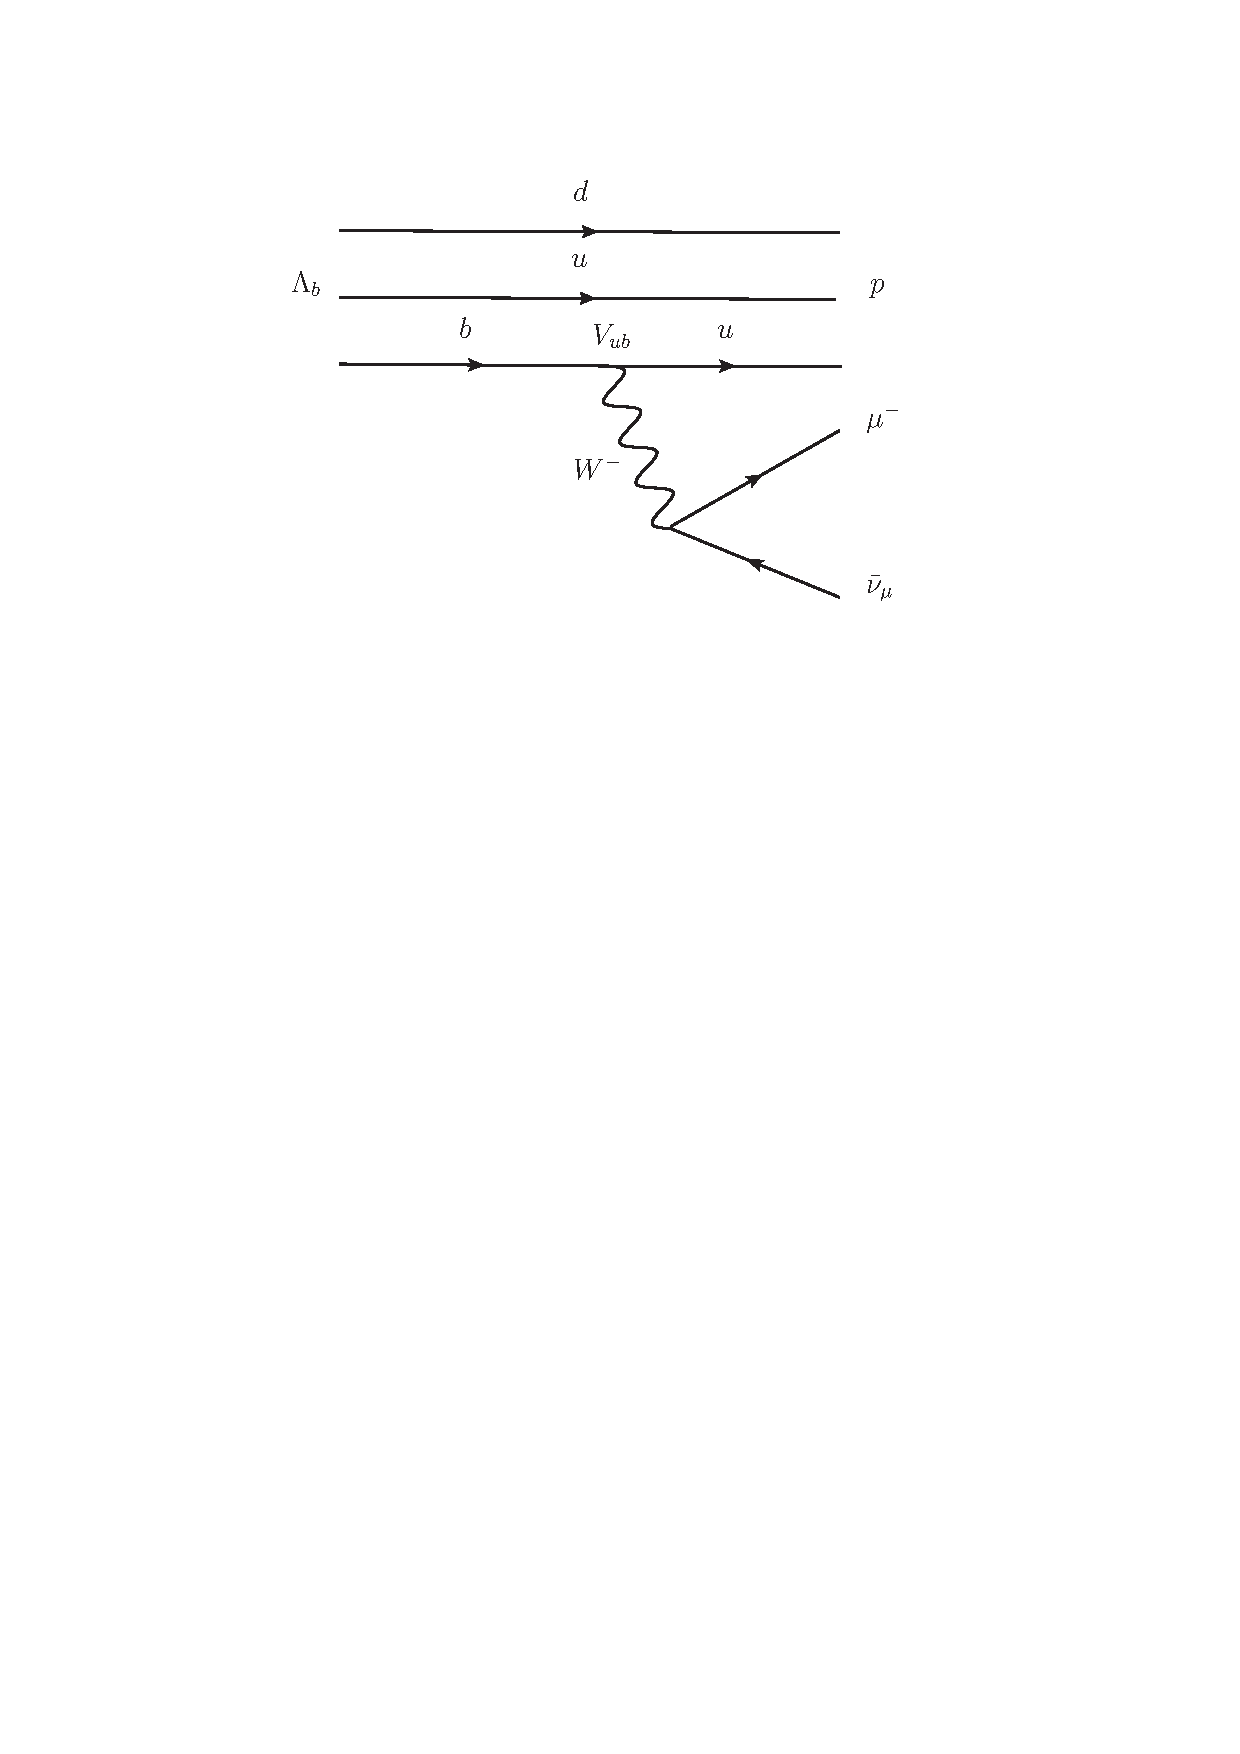
\includegraphics[trim = 15mm 190mm 0mm 30mm, clip, width=8cm]{feynsig.pdf} 
\end{center}

}

  \frame{
 \frametitle{}
\begin{itemize}
\item In general for baryon to baryon V-A transitions: $H_{\nu} =  \overline{u}_{N}(p') [ F^{V}_{1} \gamma_{\nu} + F^{V}_{2}  v_{\nu} + F^{V}_{3}  v'_{\nu} -  (F^{A}_{1} \gamma_{\nu} + F^{A}_{2}  v_{\nu} + F^{A}_{3}  v'_{\nu}) \gamma_{5}] u_{\Lambda_{b}}(p) $
\item  This convention is used by EvtGen.  Current papers presenting predictions for $\Lambda_{b} \rightarrow p$ form factors use different conventions.
\end{itemize}

\vspace{0.5cm}
For instance A. Khodjamirian et al. in arXiv:1108.2971 (LCSR predictions) use:


 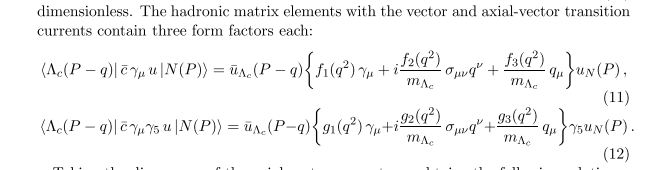
\includegraphics[width=0.9\textwidth]{def1.png} 

}

  \frame{
 \frametitle{}
Meanwhile W. Detmold, S. Meinel et al. in arXiv:1306.0446 (LQCD predictions) use the form:
\vspace{0.25cm}
 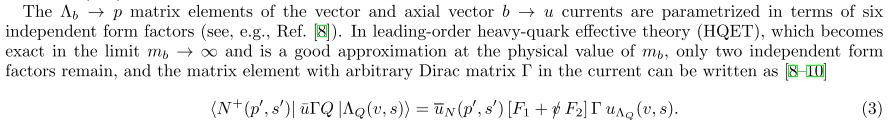
\includegraphics[width=1.0\textwidth]{def2.png} 
 \begin{itemize}
\item Use HQET under which only 2 form factors are required.
\end{itemize}


}

  \frame{
 \frametitle{}
Also include next to first order loop corrections:
\vspace{0.25cm}
 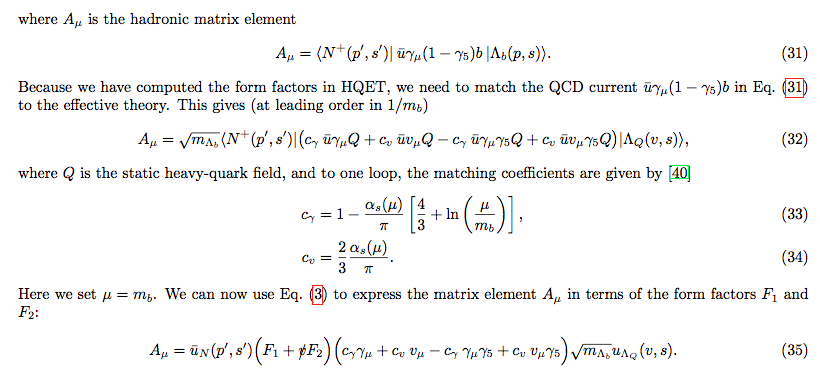
\includegraphics[width=1.\textwidth]{def3.png} 



}

  \frame{
 \frametitle{}
  \begin{itemize}
\item Need to match the form factors calculated in arXiv:1108.2971 (LCSR predictions) and  arXiv:1306.0446 (LQCD predictions) to convention used by EvtGen.
\item Contacted Stefan Meinel (theorist at MIT) and he kindly provided me with a number of derivations relating the various from factors.
 \end{itemize}

}


  \frame{
 \frametitle{Generator level MC}
 Now compare generator level distributions for LQCD, LCSR and Phase Space predictions:
      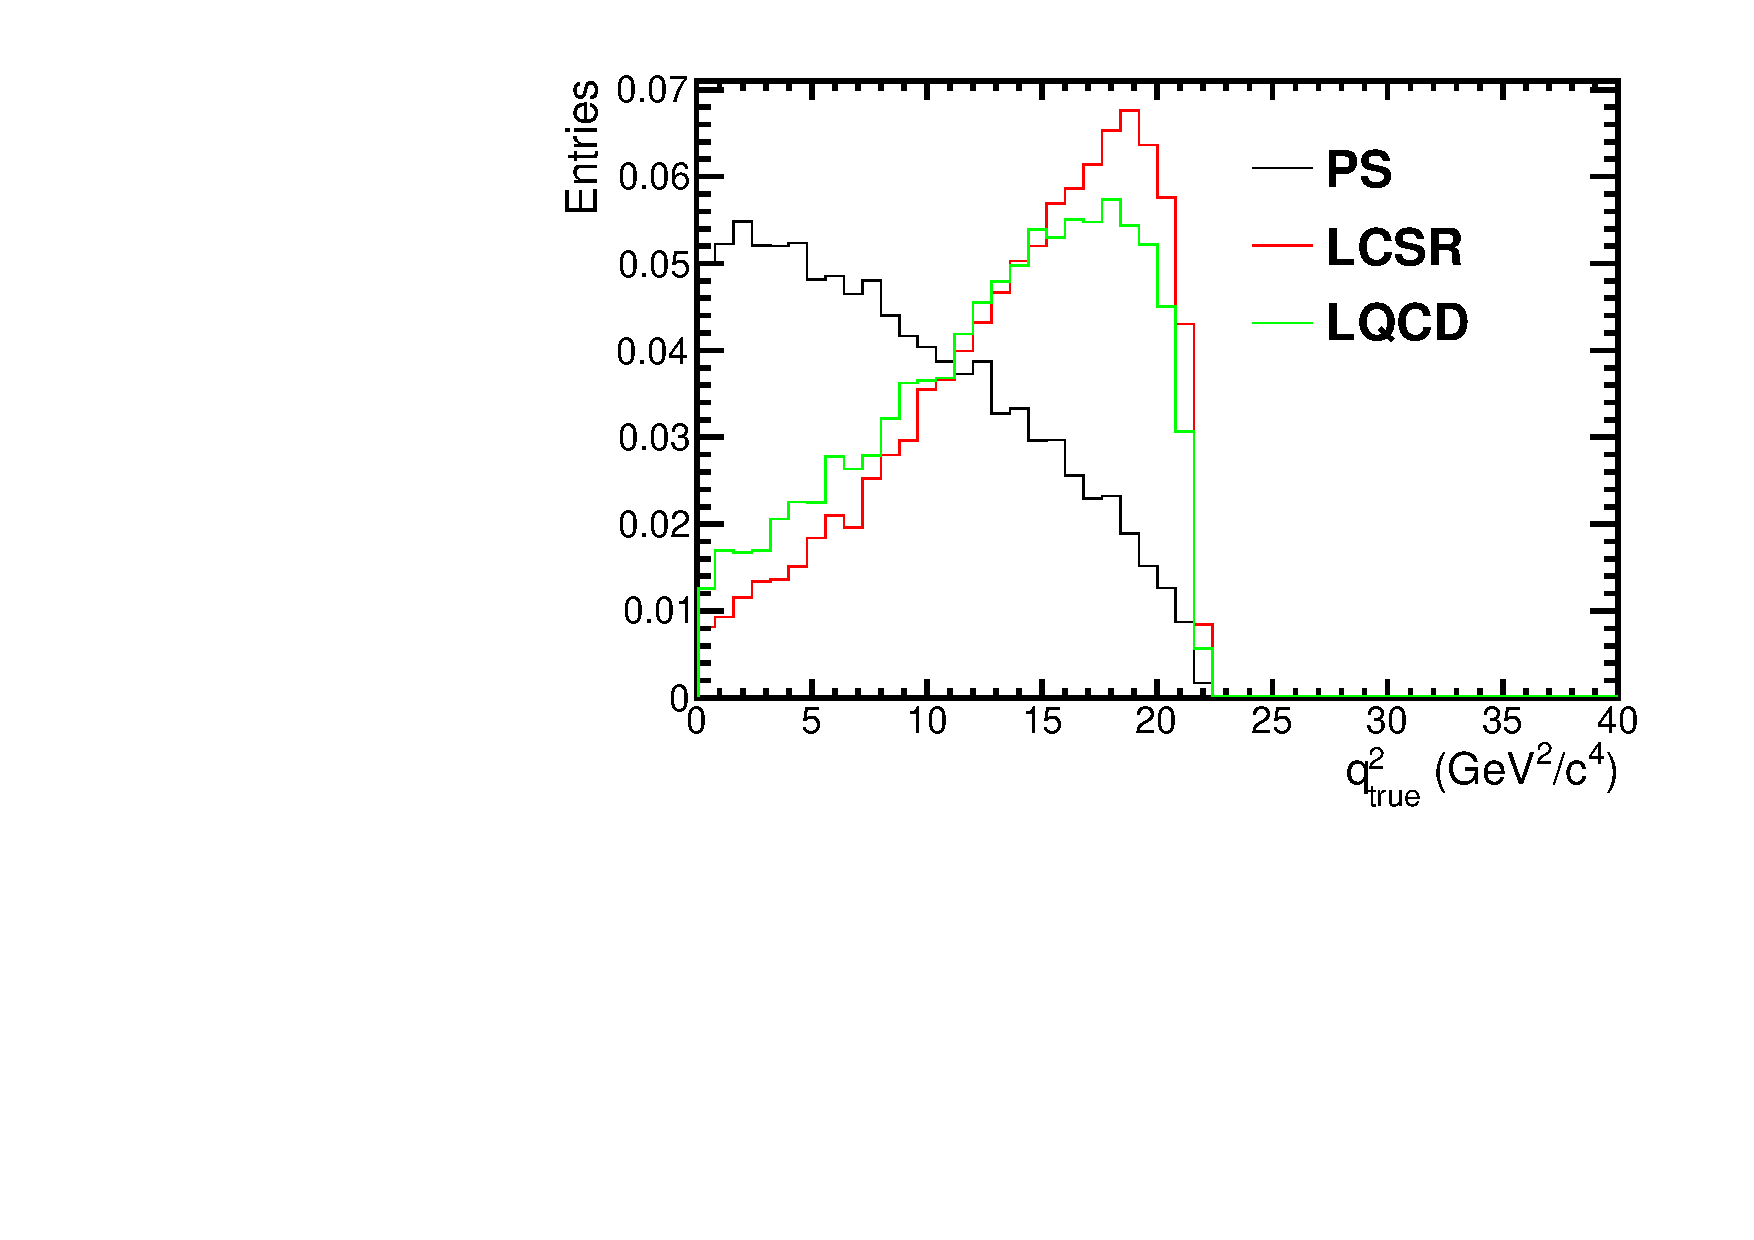
\includegraphics[width=0.4\textwidth]{PSpace_q2vsX/q2_trueSIG.pdf}    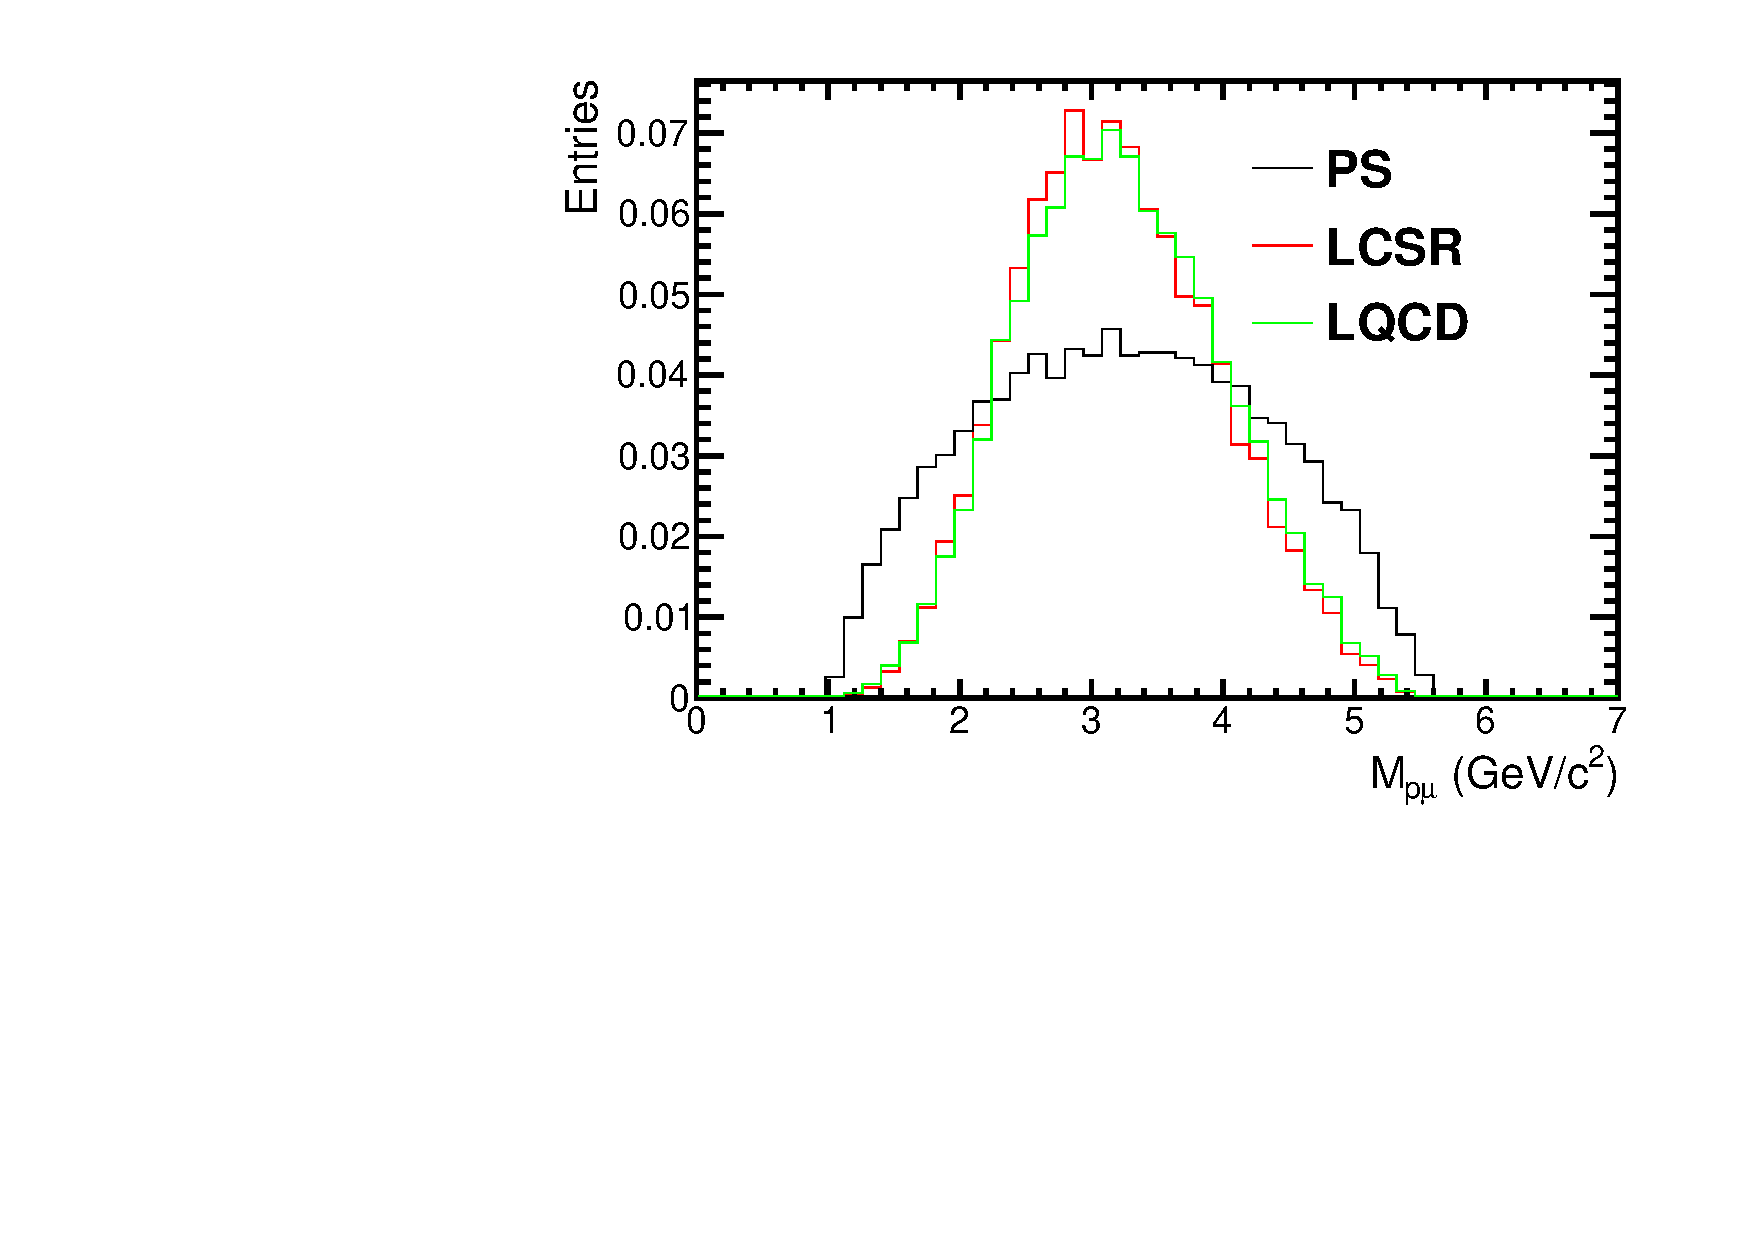
\includegraphics[width=0.4\textwidth]{PSpace_q2vsX/M_pmuSIG.pdf} \\
     
       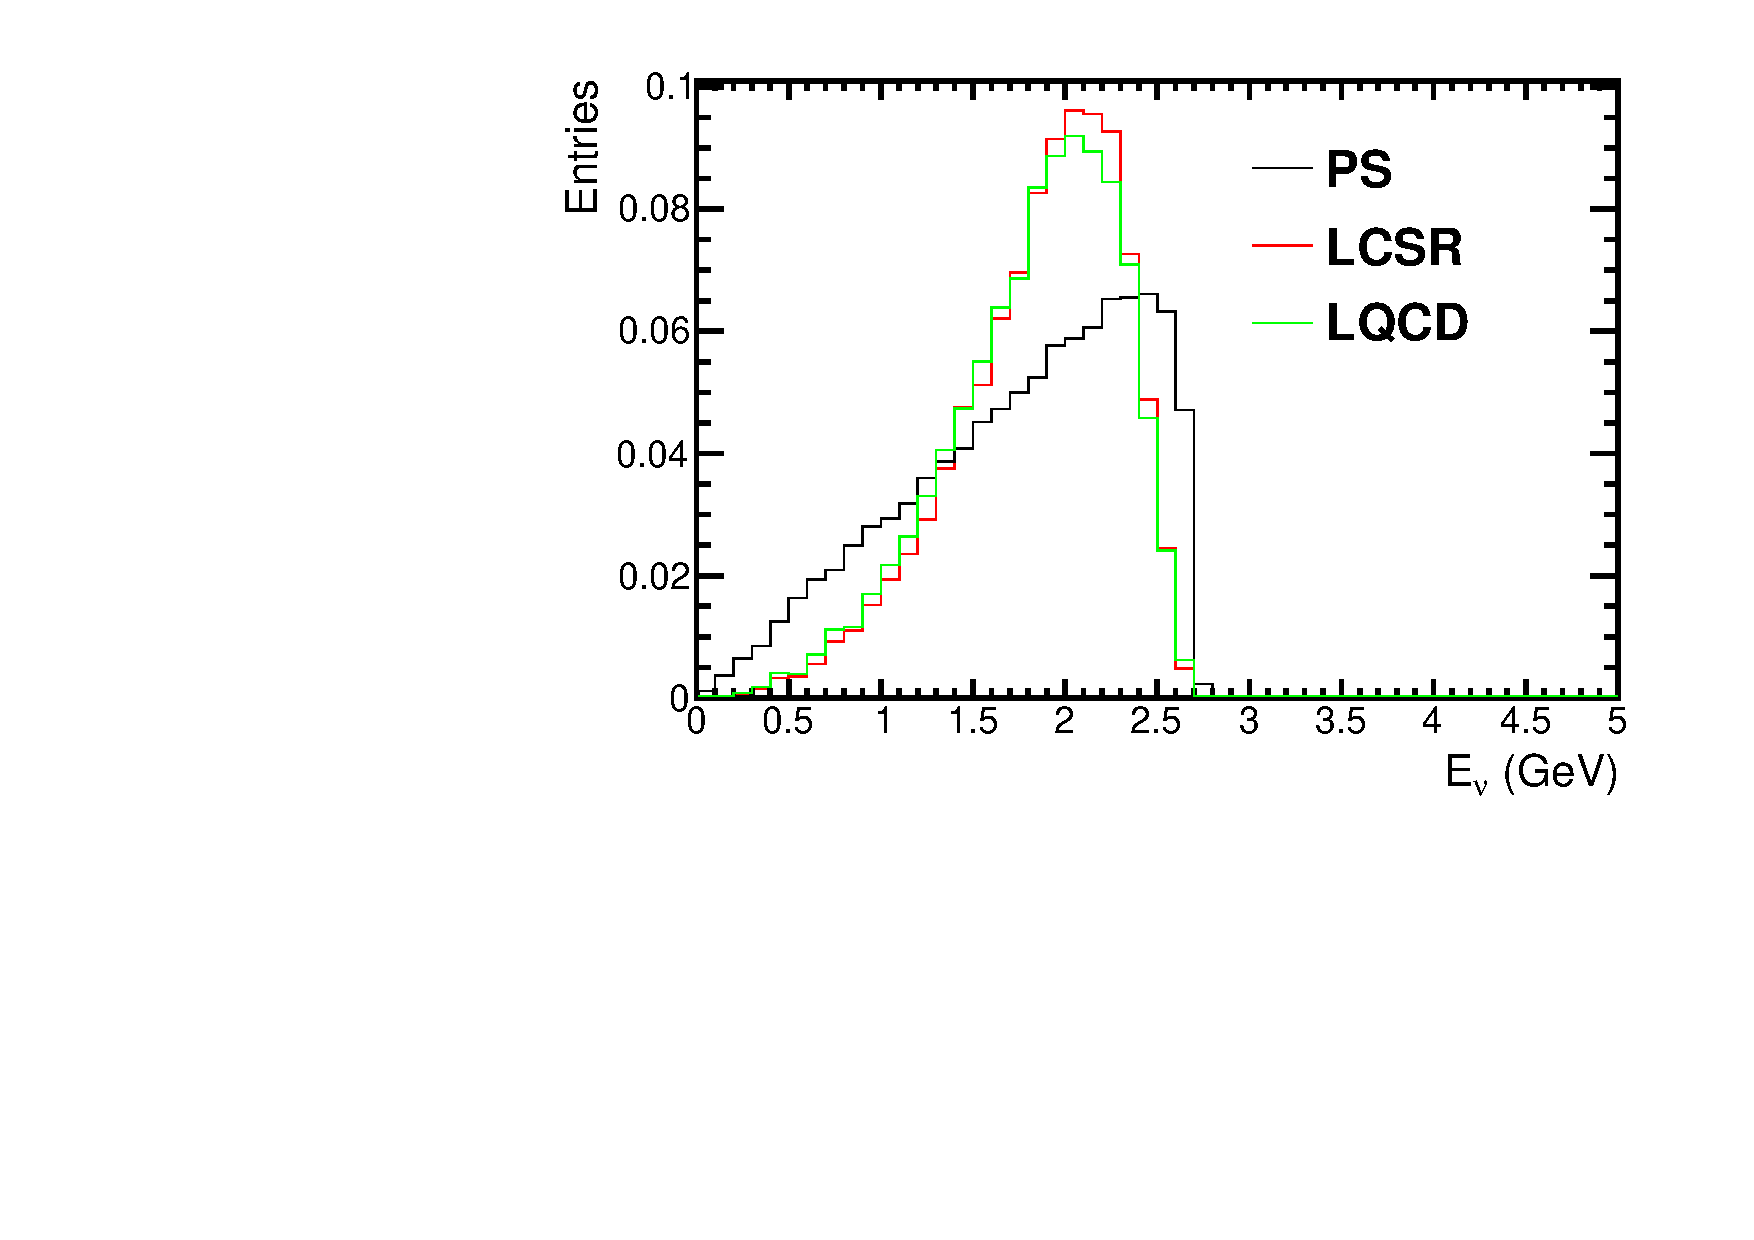
\includegraphics[width=0.4\textwidth]{PSpace_q2vsX/E_nuSIG.pdf}    
       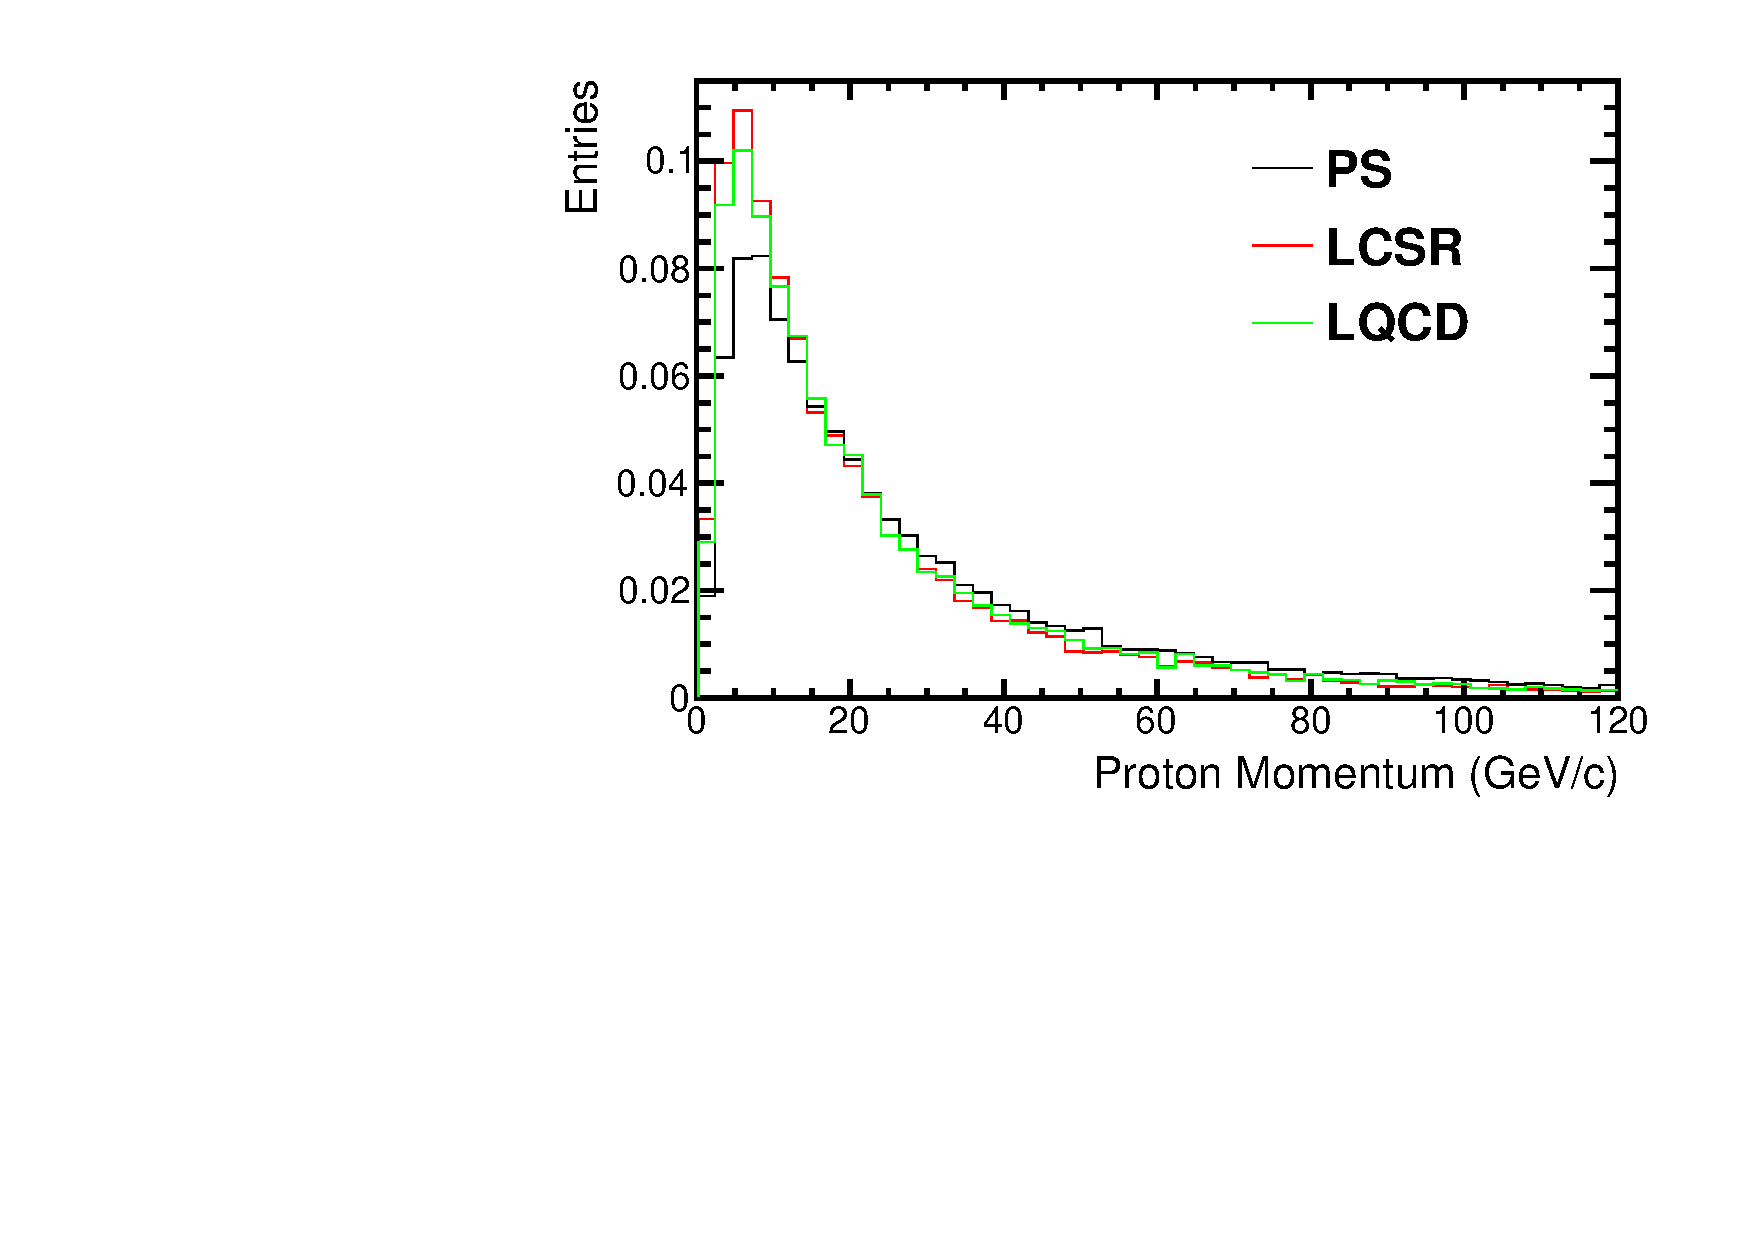
\includegraphics[width=0.4\textwidth]{PSpace_q2vsX/P_ProtonSIG.pdf} 
}

  \frame{
 \frametitle{}
  \hspace{2cm}  \uline{LCSR}  \hspace{4cm} \uline{Phase Space}
      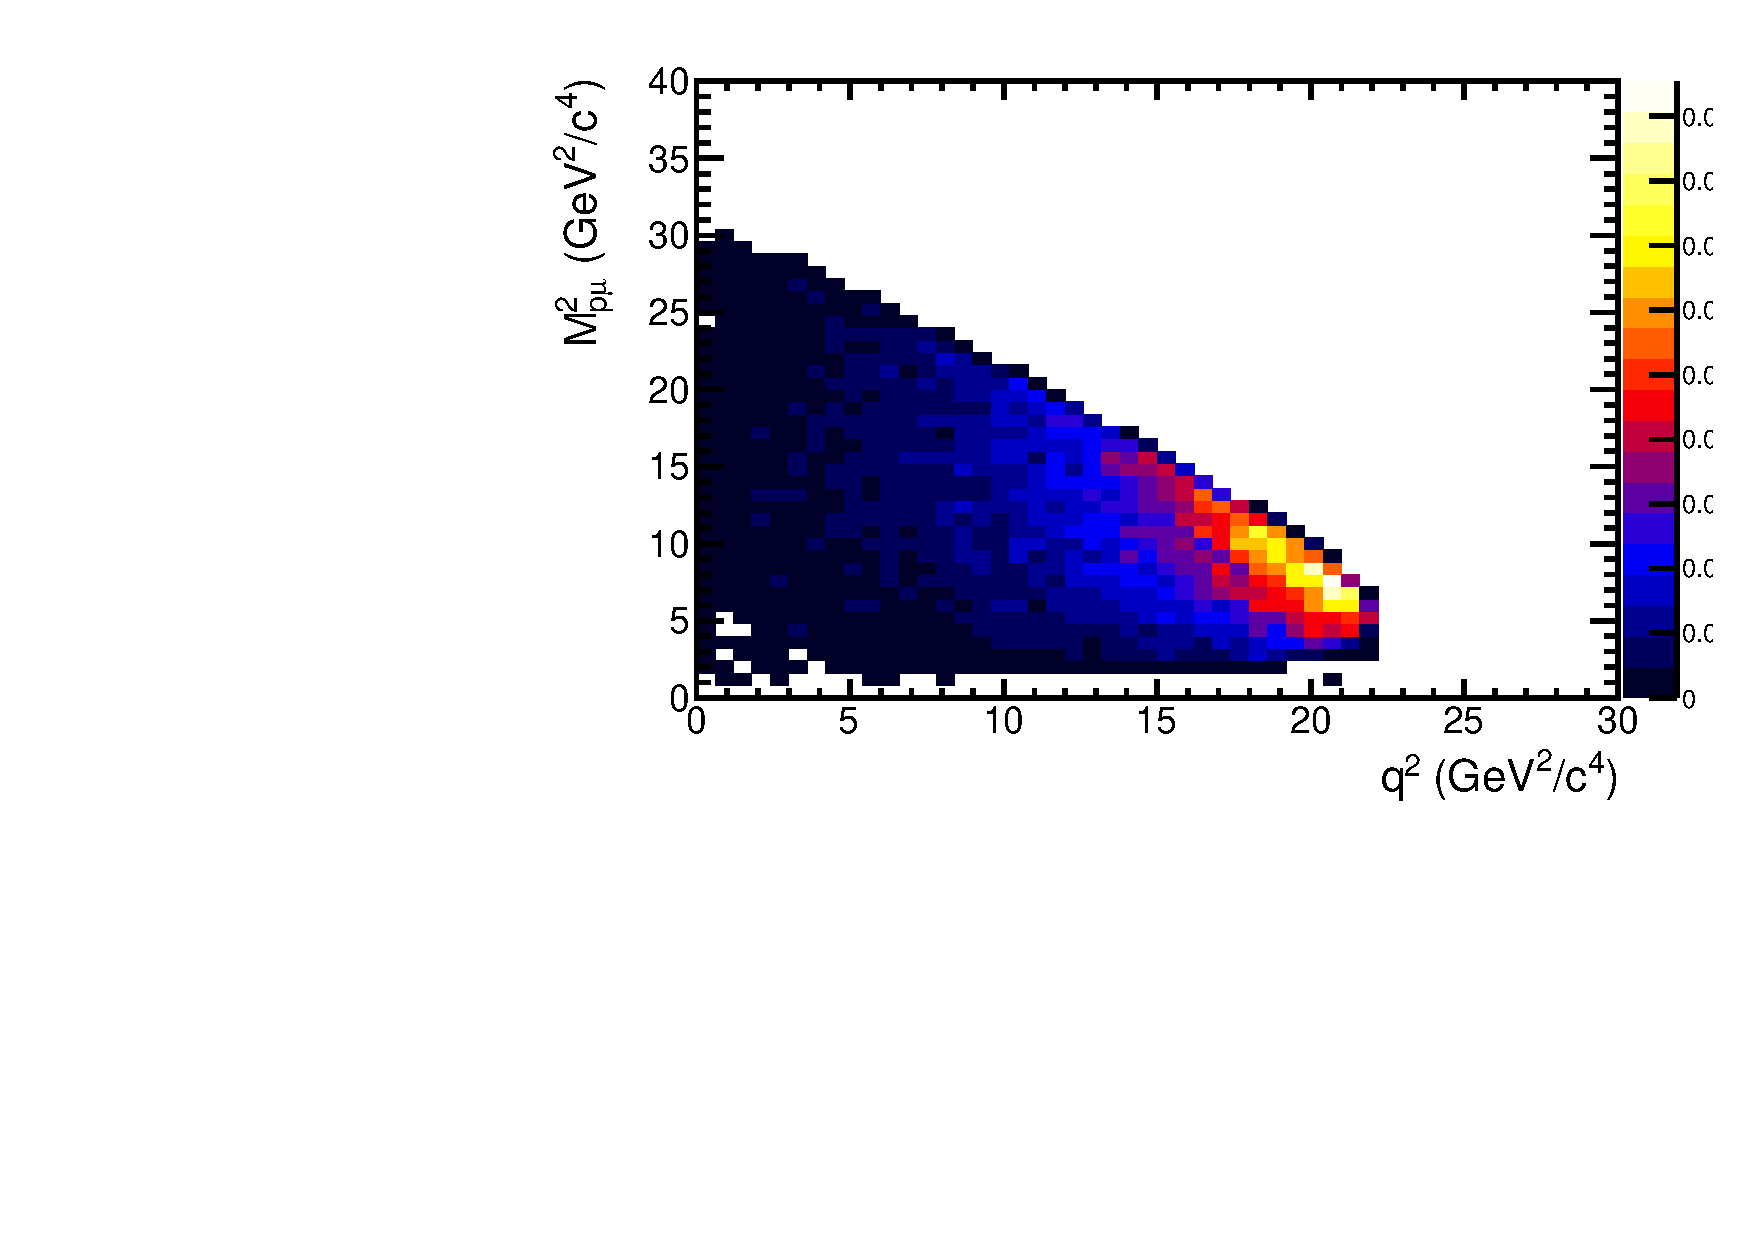
\includegraphics[width=0.45\textwidth]{LCSR_q2vsX/M_pmu.pdf}    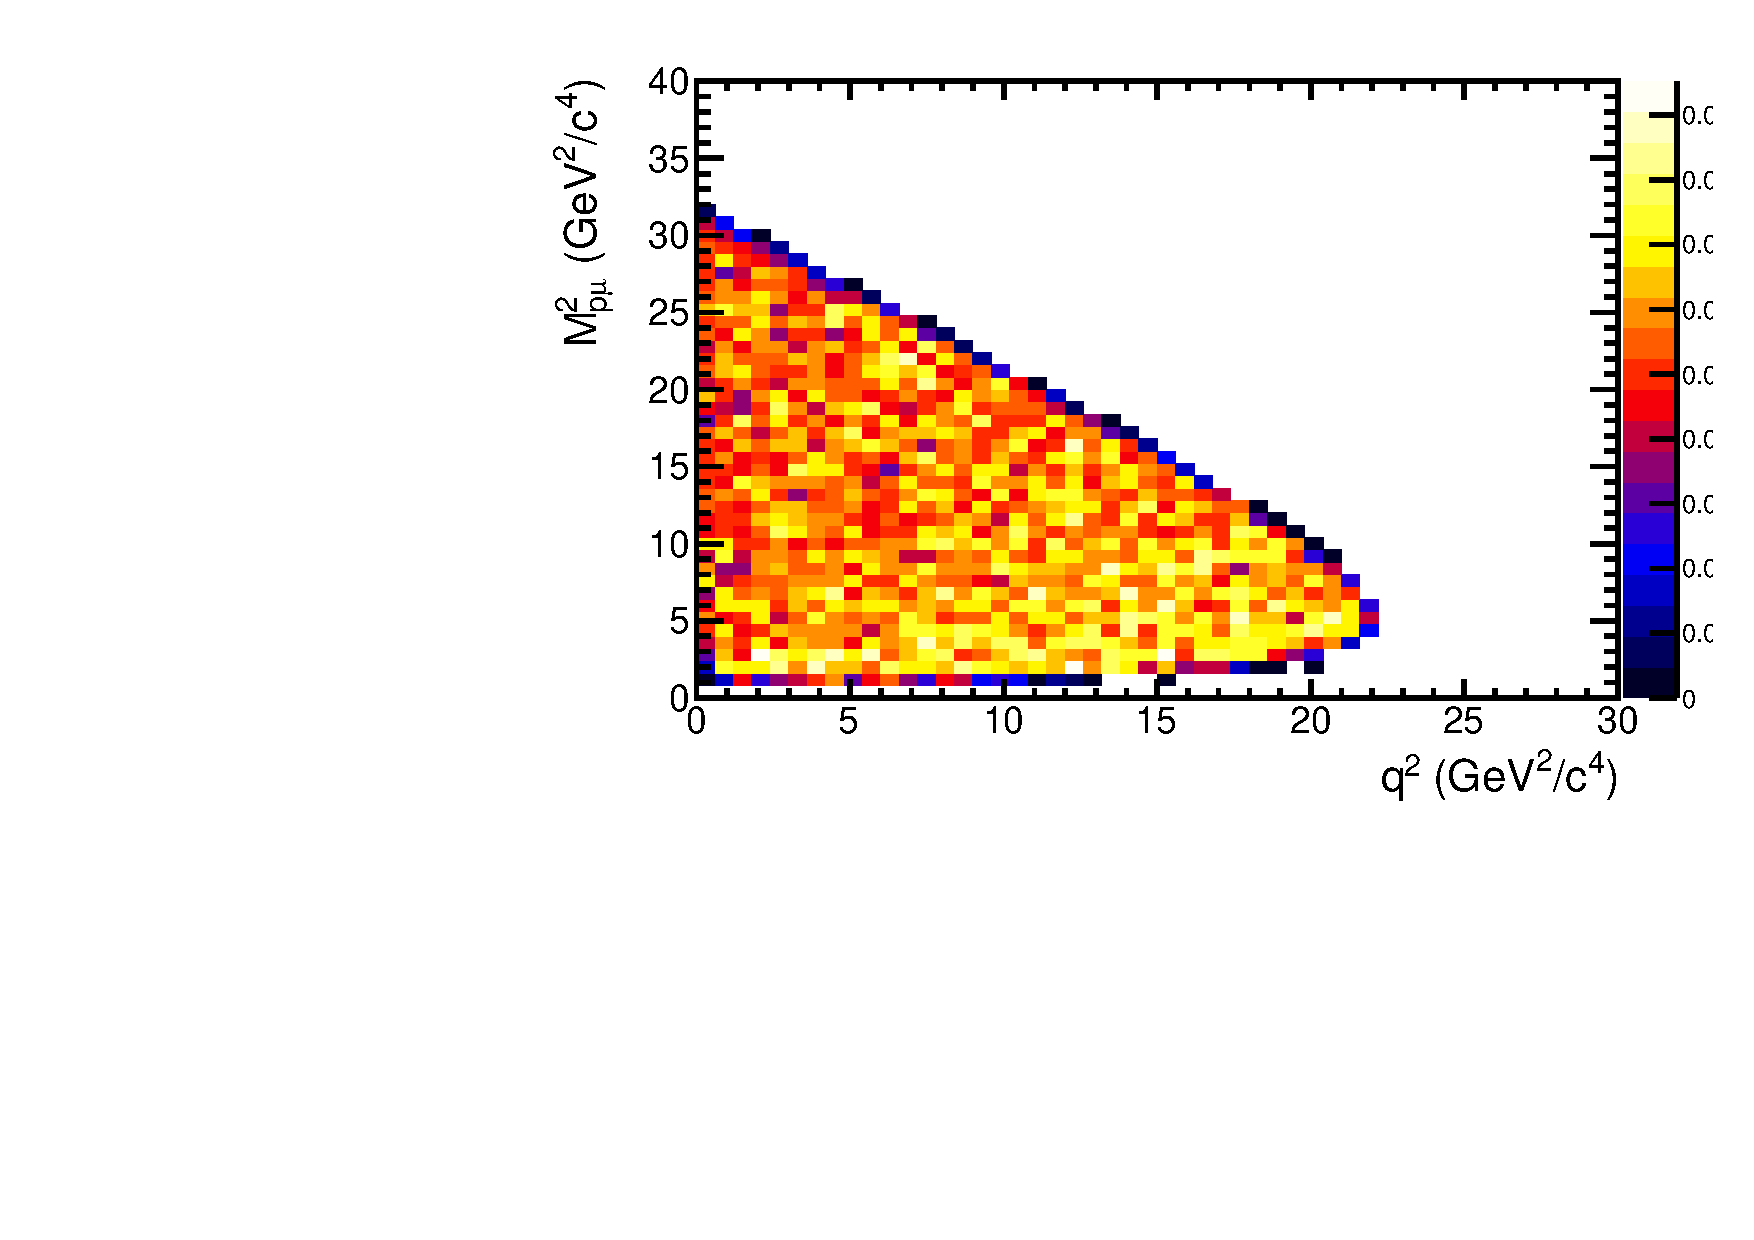
\includegraphics[width=0.45\textwidth]{PSpace_q2vsX/M_pmu.pdf} \\
      \begin{center}
      \uline{LQCD}\\
       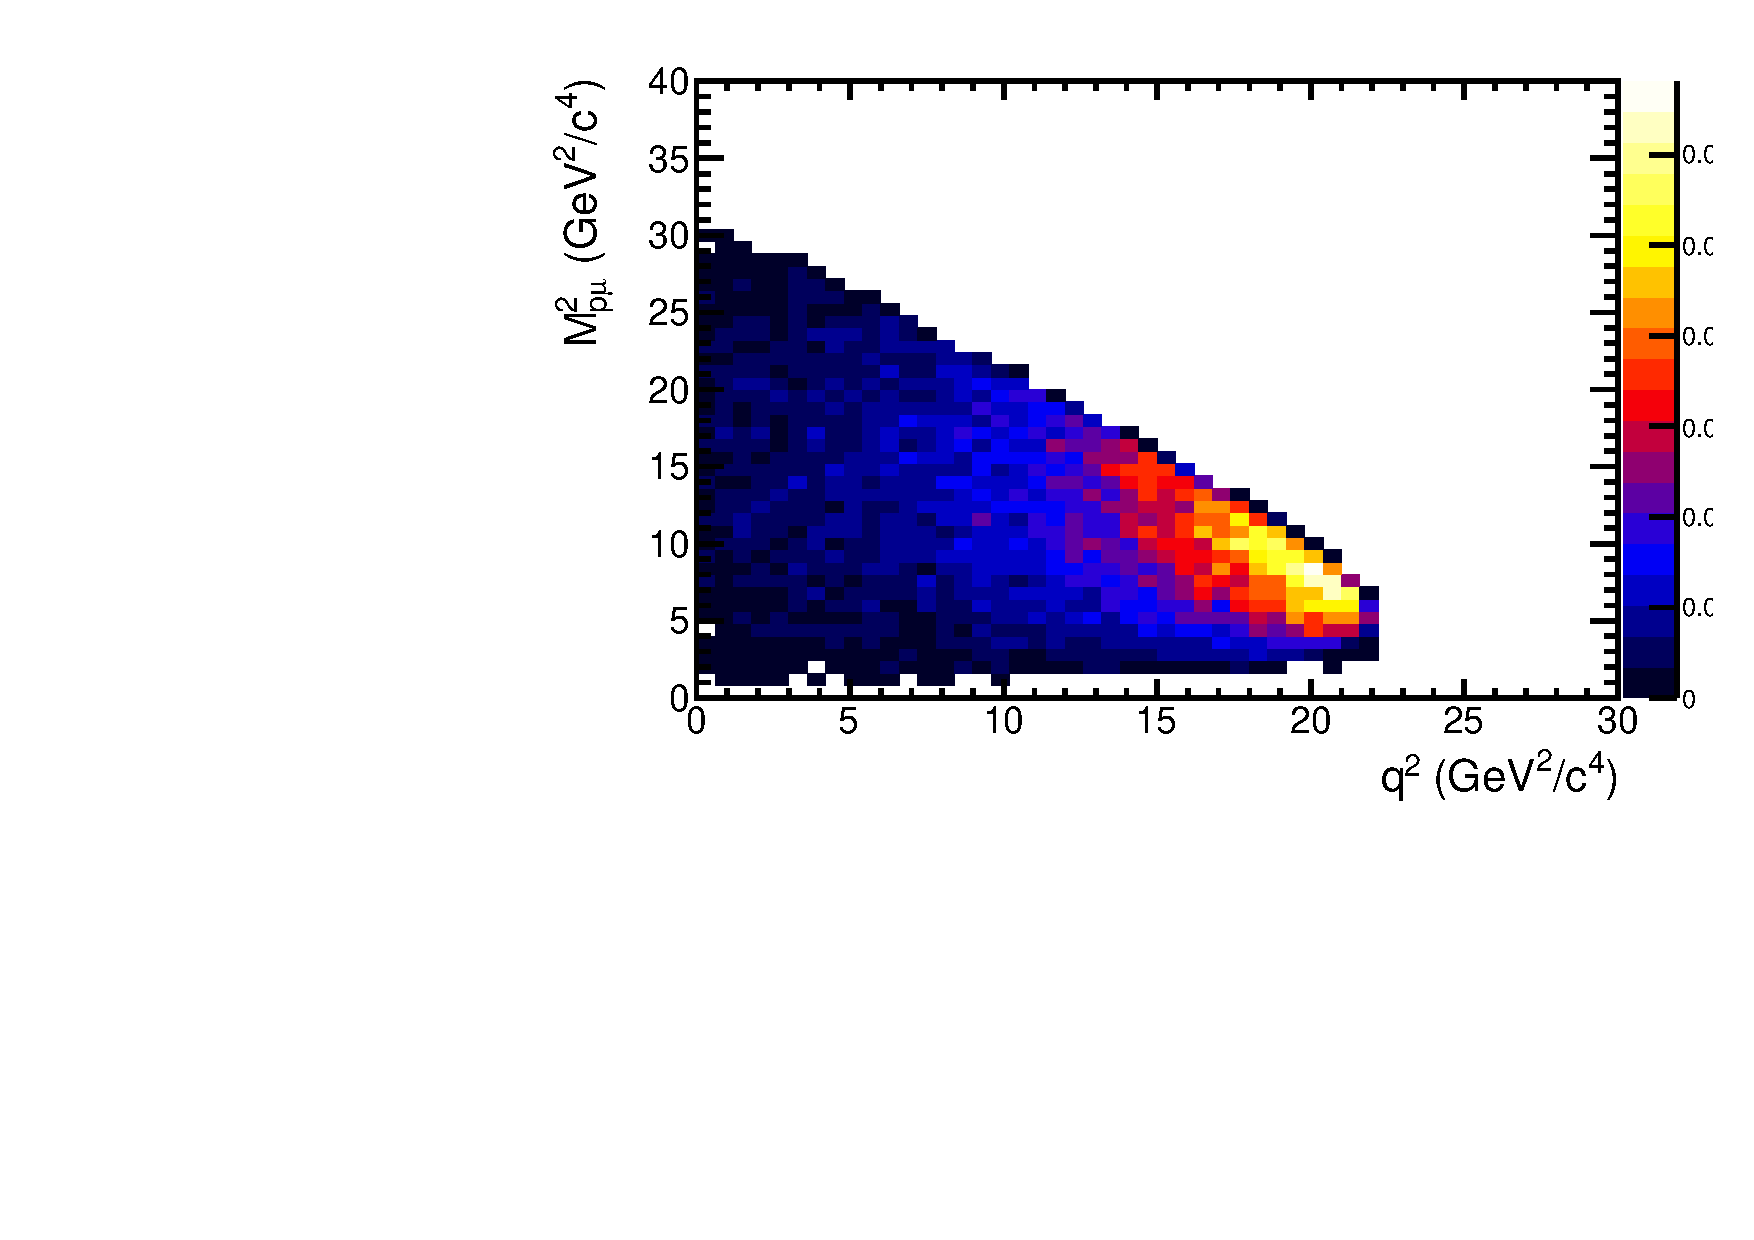
\includegraphics[width=0.45\textwidth]{LQCD_q2vsX/M_pmu.pdf}   
       \end{center}
     
    }


  \frame{
 \frametitle{}
  \begin{itemize}
\item Consistency check for these distributions?
\item Can at least compare the $q^{2}$ distributions with the predicted differential rate, which is derived in terms of the various form factors in both papers.
 \end{itemize}
  \hspace{0.5cm}  \uline{LCSR, arXiv:1108.2971}  \hspace{1cm} \uline{LQCD, arXiv:1306.0446}\\
  \hspace{0.5cm}  \uline{A. Khodjamirian et al.}  \hspace{1cm} \uline{W. Detmold et al.}
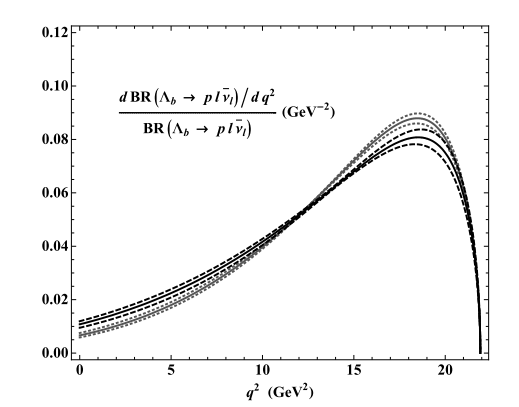
\includegraphics[width=0.45\textwidth]{LCSR.png} 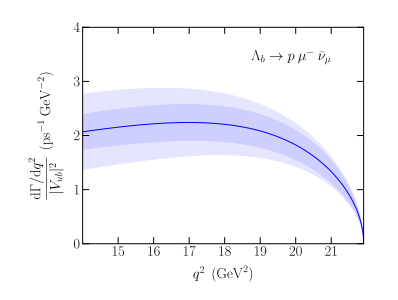
\includegraphics[width=0.5\textwidth]{LQCD.png} 

}

  \frame{
 \frametitle{}
 For LQCD: \\
 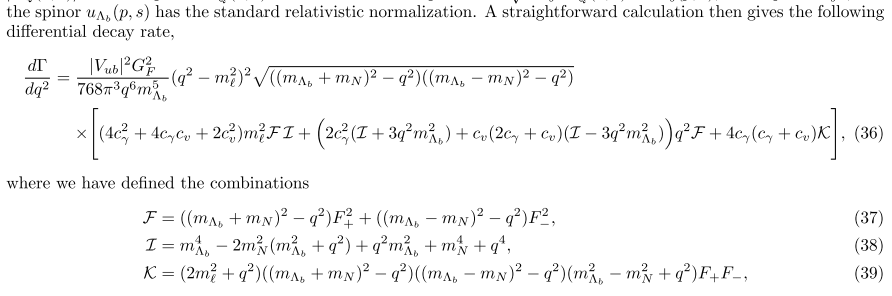
\includegraphics[width=0.8\textwidth]{def4.png}\\
For LCSR: \\
 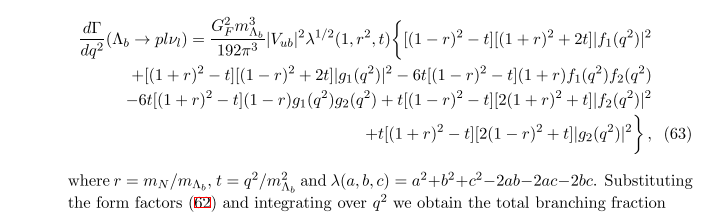
\includegraphics[width=0.8\textwidth]{def5.png}
}


  \frame{
 \frametitle{}
  \begin{itemize}
\item Make 2 new RooPdf classes for LCSR and LQCD differential BF predictions.
\item Can then fit these to the generator level $q^{2}$ distribution.
\item Only leave normalisation free.
 \end{itemize}

}
  \frame{
 \frametitle{}
  \begin{itemize}
  \item Generate 100,000 MC toys using the theoretically predicted differential BF.
  \item Here LCSR (red) and LQCD (blue):
 \end{itemize}
 

 \vspace{0.2cm}
\begin{center}
       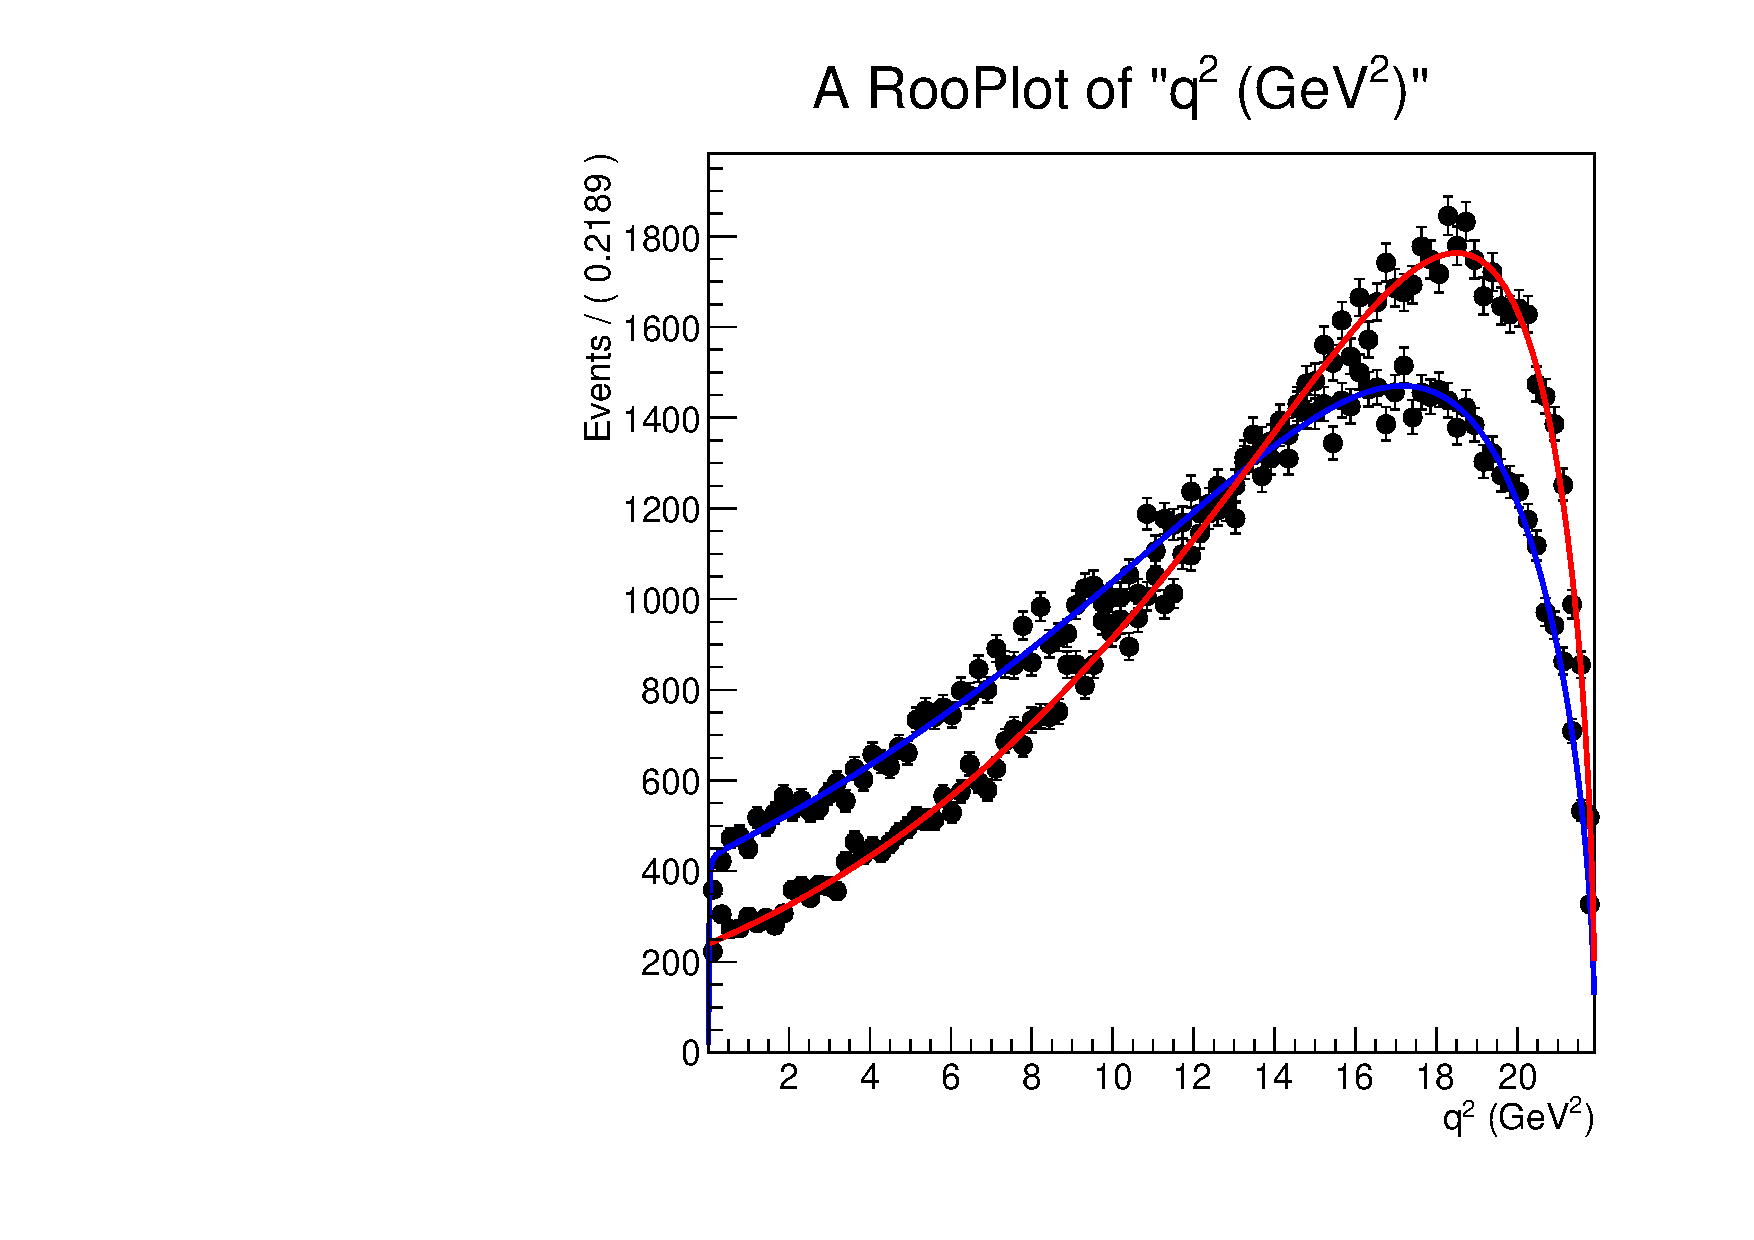
\includegraphics[width=0.6\textwidth]{plot.pdf} 
     \end{center}
    
}


  \frame{
 \frametitle{}
 Fit generator level data: \\
 \vspace{0.5cm}
  \hspace{2cm}  \uline{LQCD}  \hspace{4cm} \uline{LCSR}
      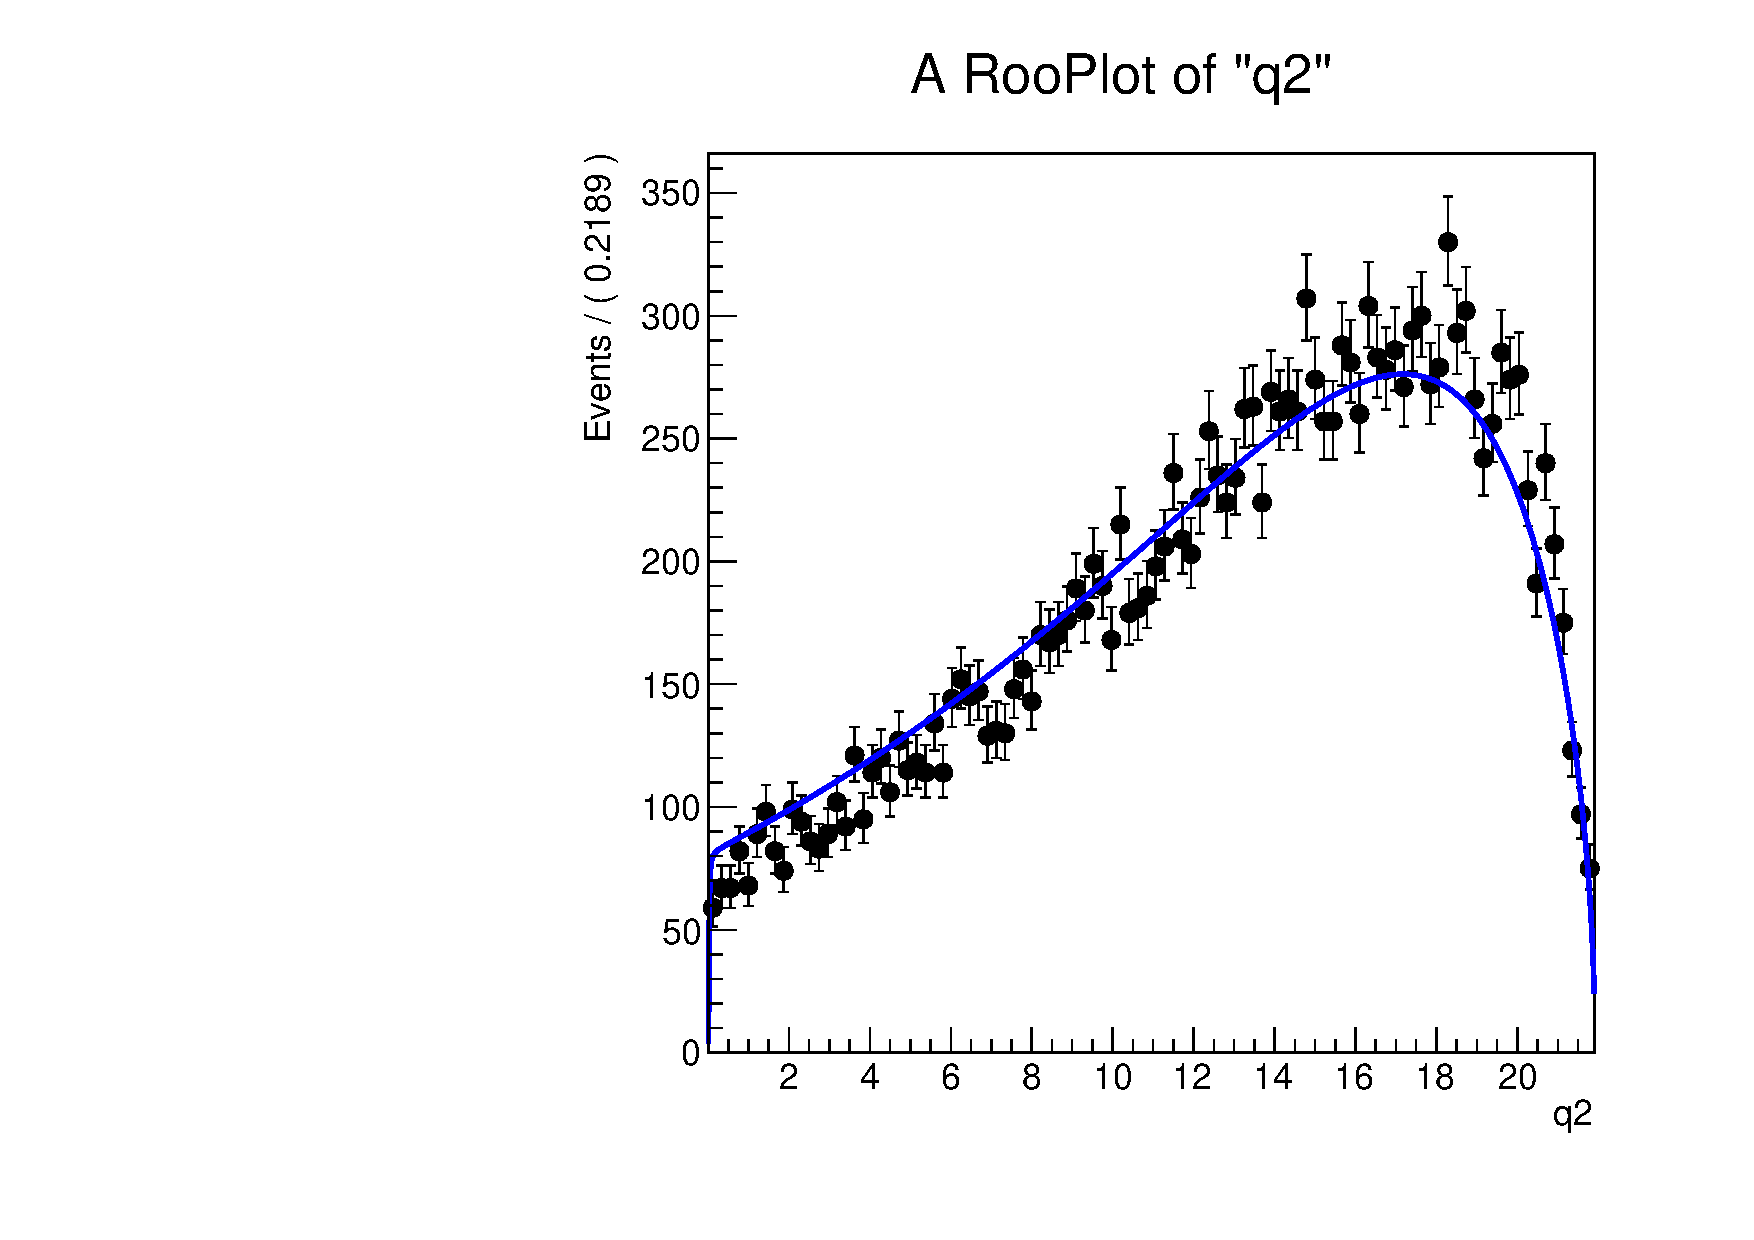
\includegraphics[width=0.5\textwidth]{Roo_q2plot.pdf}    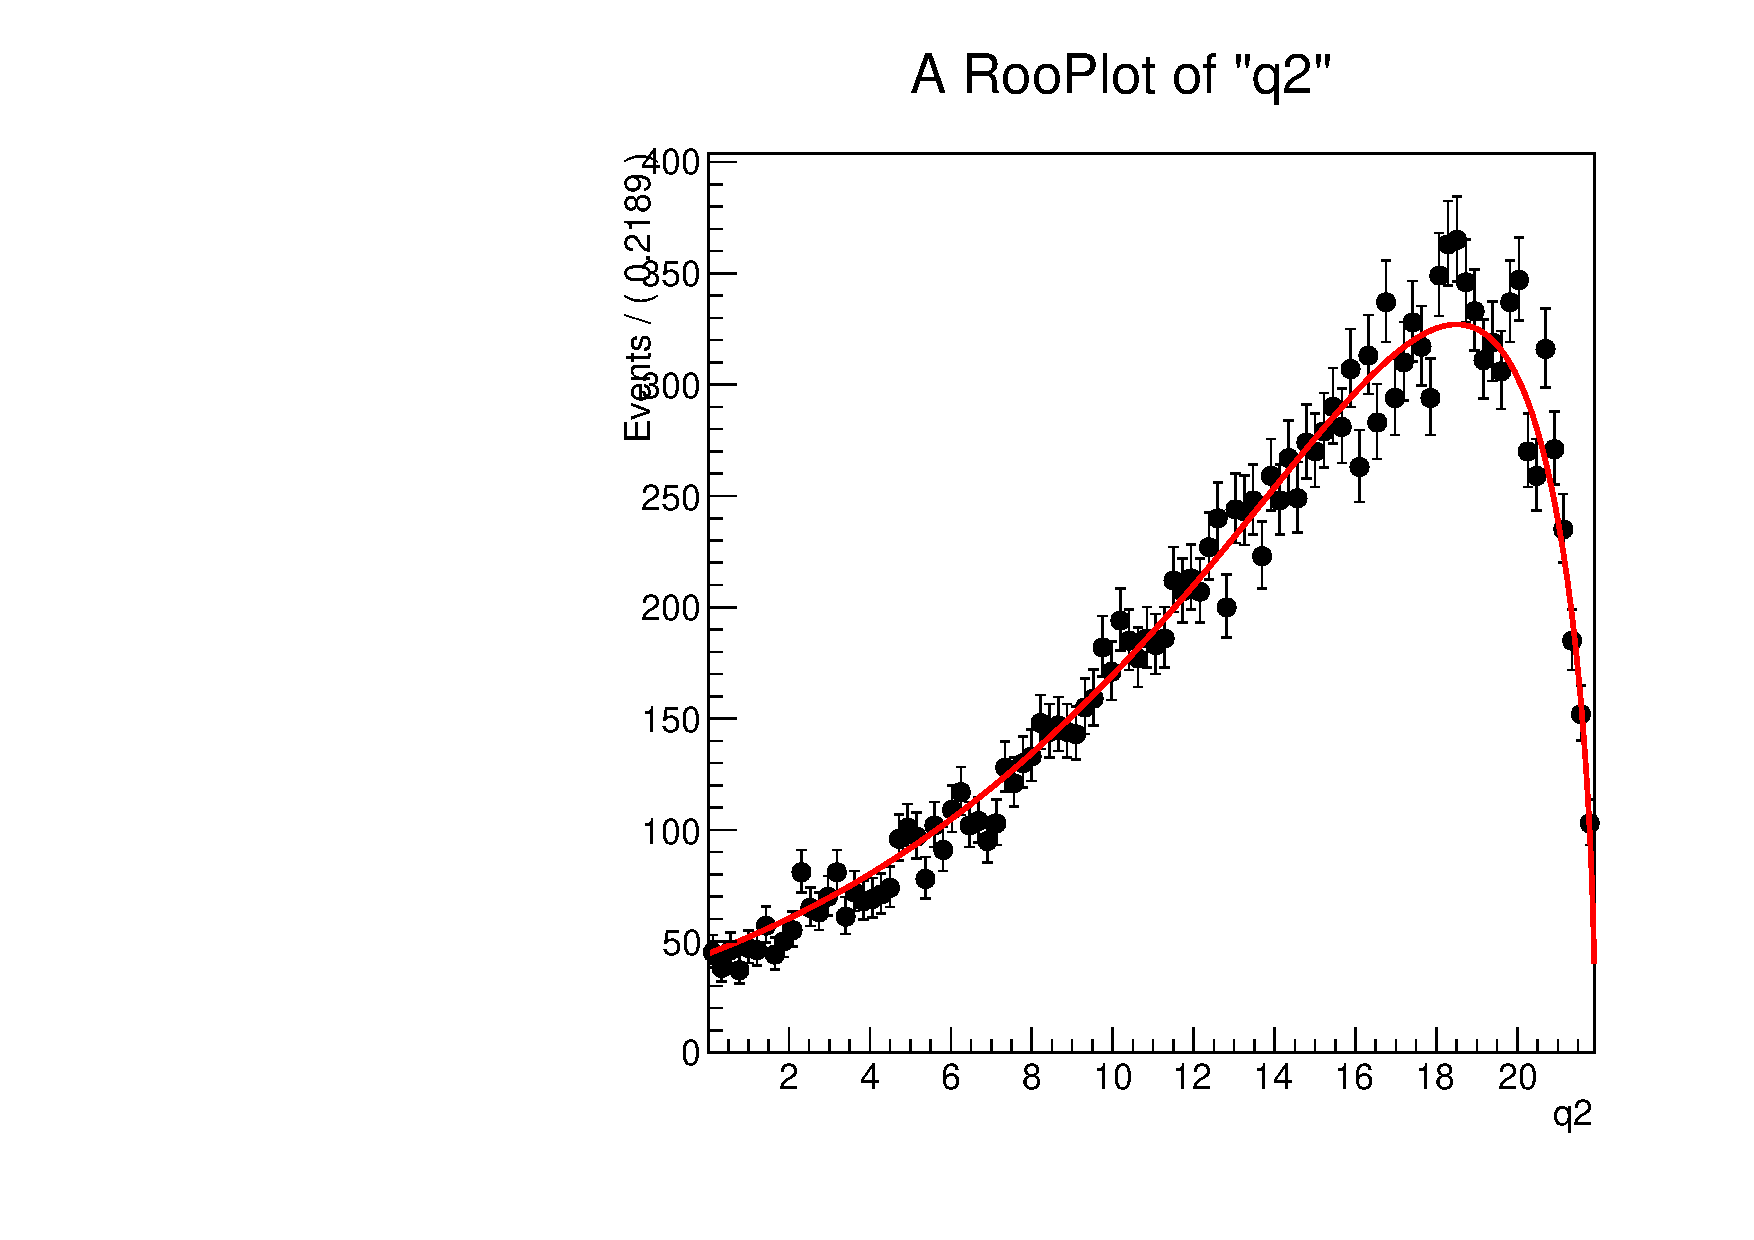
\includegraphics[width=0.5\textwidth]{Roo_q2plot_LCSR.pdf} \\
     
    
}


%%%%new section
\section{Conclusion}
  \frame{
 \frametitle{Conclusion}
 \begin{itemize}
  \setlength{\itemsep}{5pt}
  

  \item Thanks to Stefan Meinel have relations between the form factors defined by EvtGen and those defined in papers.
    \item Plots seem to make sense.
     \item However, LQCD fit is not perfect.  Further checks + greater statistics required.
   \item Need to get changes into EvtGen soon so I can get new and improved MC
   \end{itemize}

}

}
 \end{document}